\chapter{Circular Experiment}

Workers were asked where the circle was compared to a point in the image.
The circle was placed in 32 positions, with the angle between the dot and circle being varied. Each worker was asked to provide 16 responses.

Originally the workers were asked to provide all 32 responses, but no workers decided to  do this. 
It is unclear if this was due to the number of questions being asked, which was relatively high for each worker, or if it was another issue such as the time of posting the task. 




%Raw dataset
\begin{figure}
	\centering
	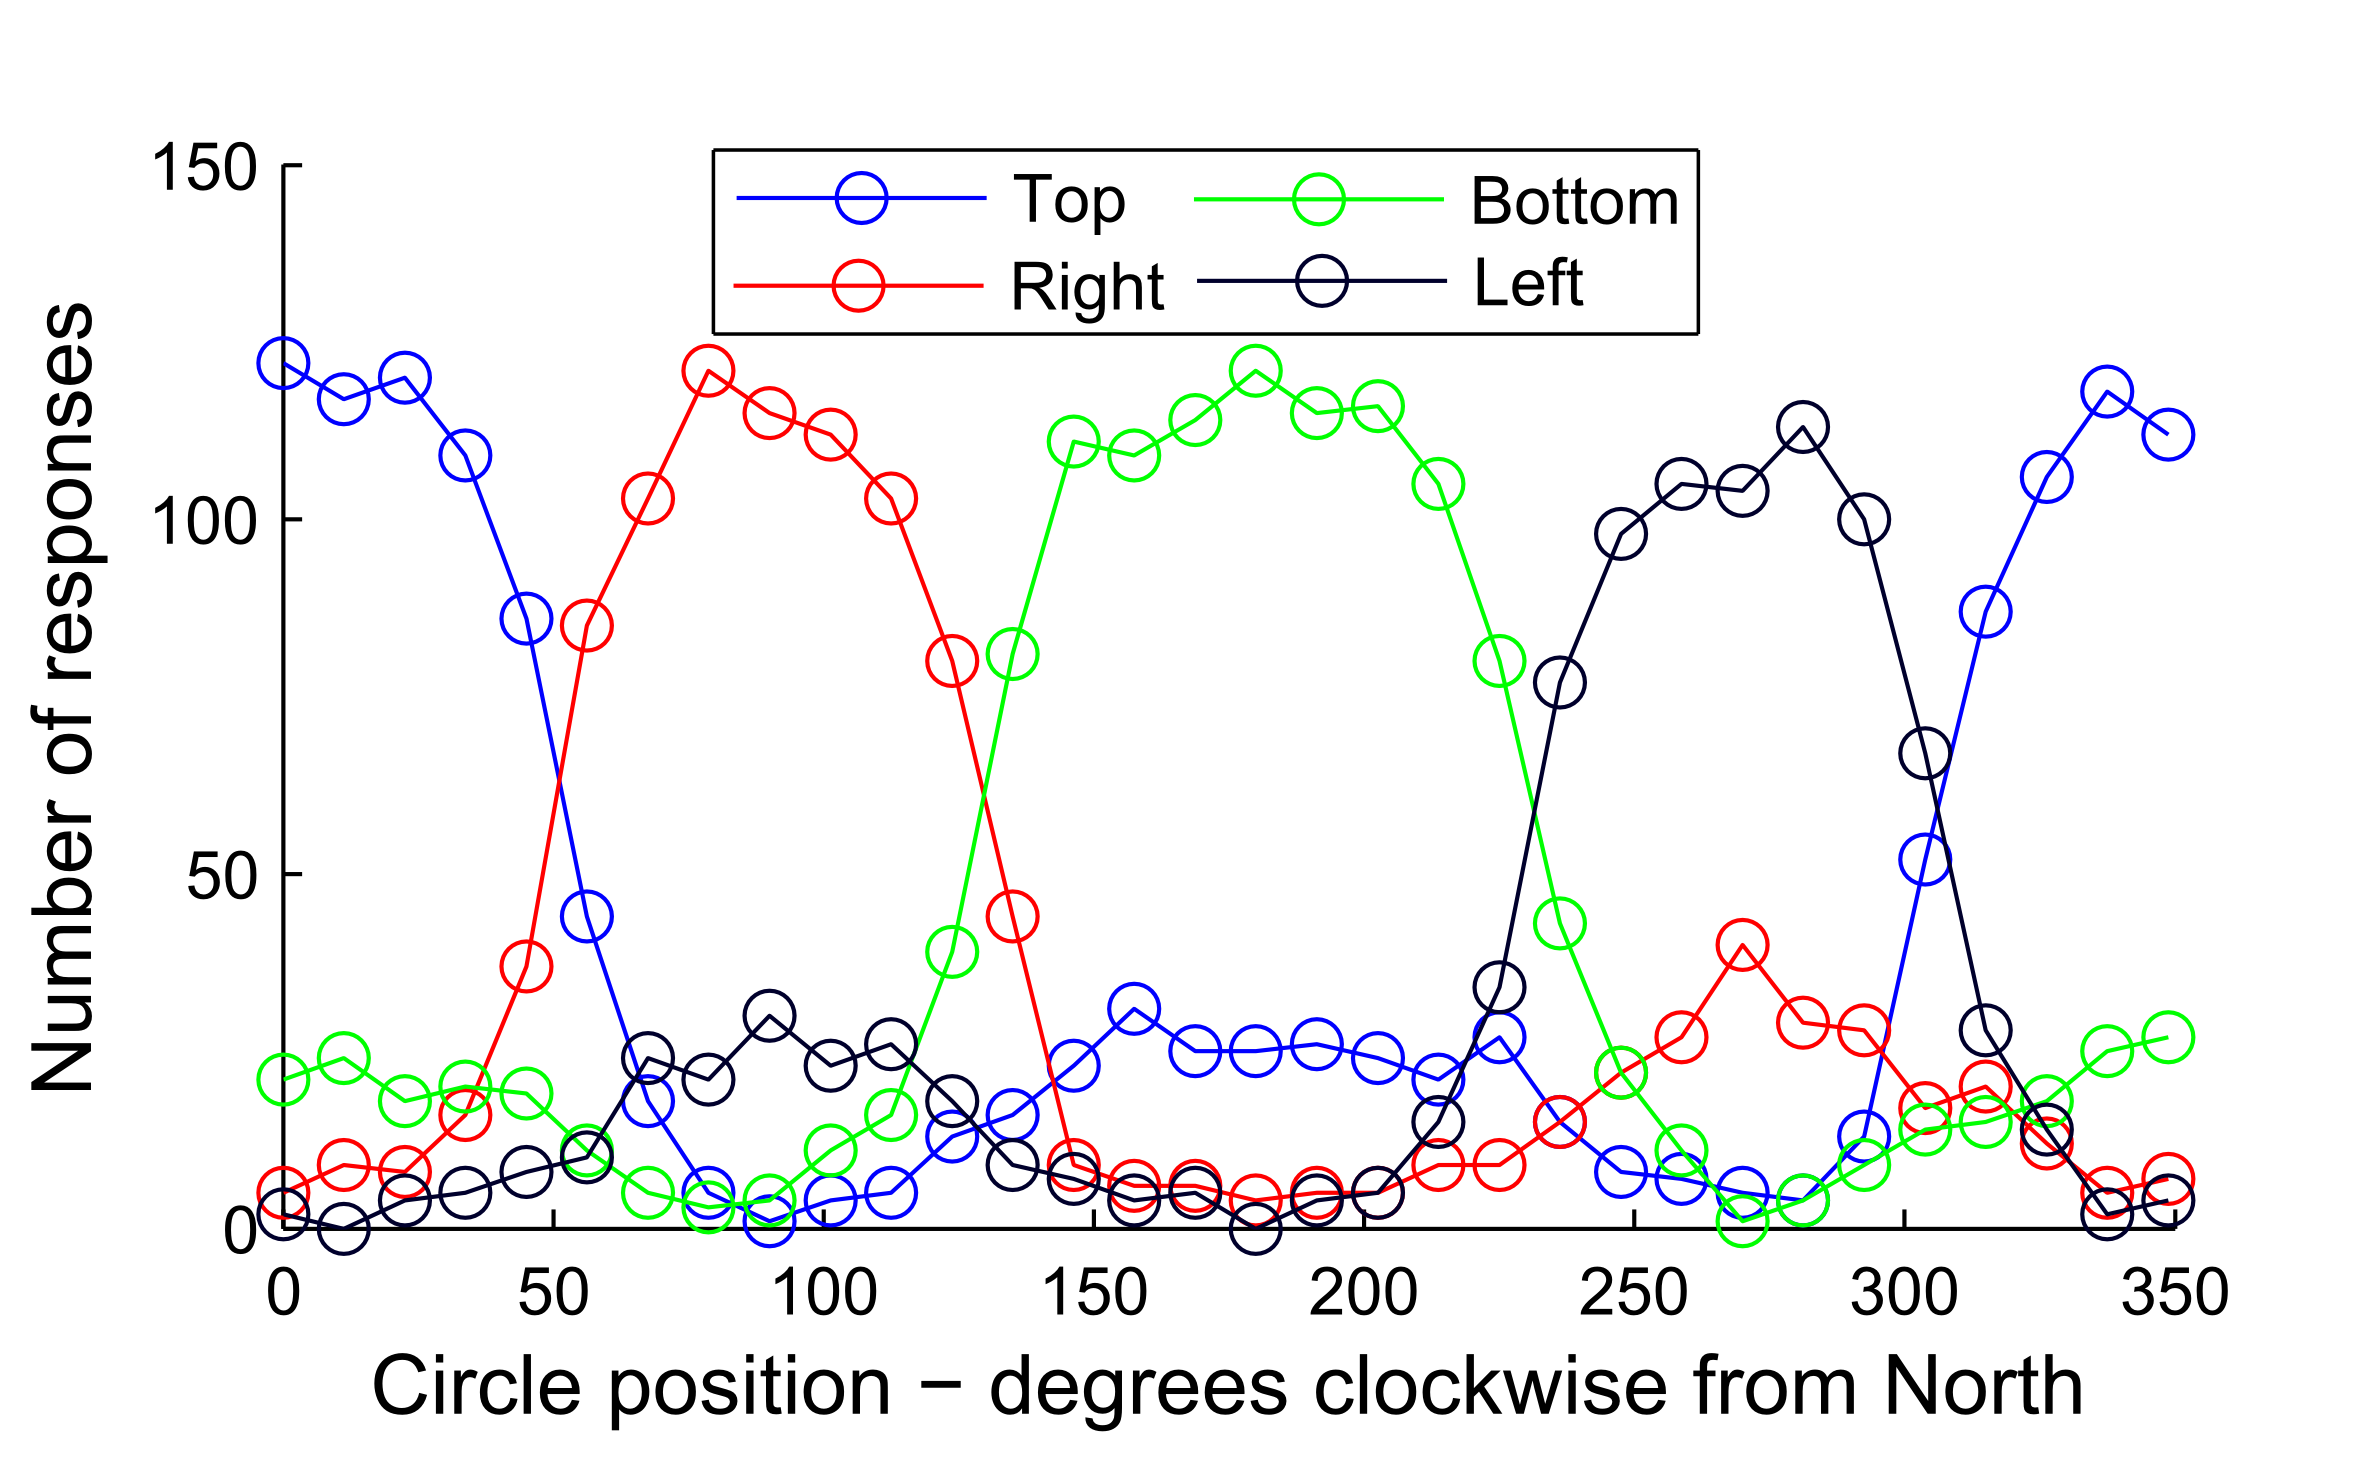
\includegraphics[scale=1]{line_circular_raw_data.png}
	\caption{The number of responses at each of the 32 circle positions}
	\label{Figure:circular_raw_responses}
\end{figure}

\begin{figure}
	\centering
	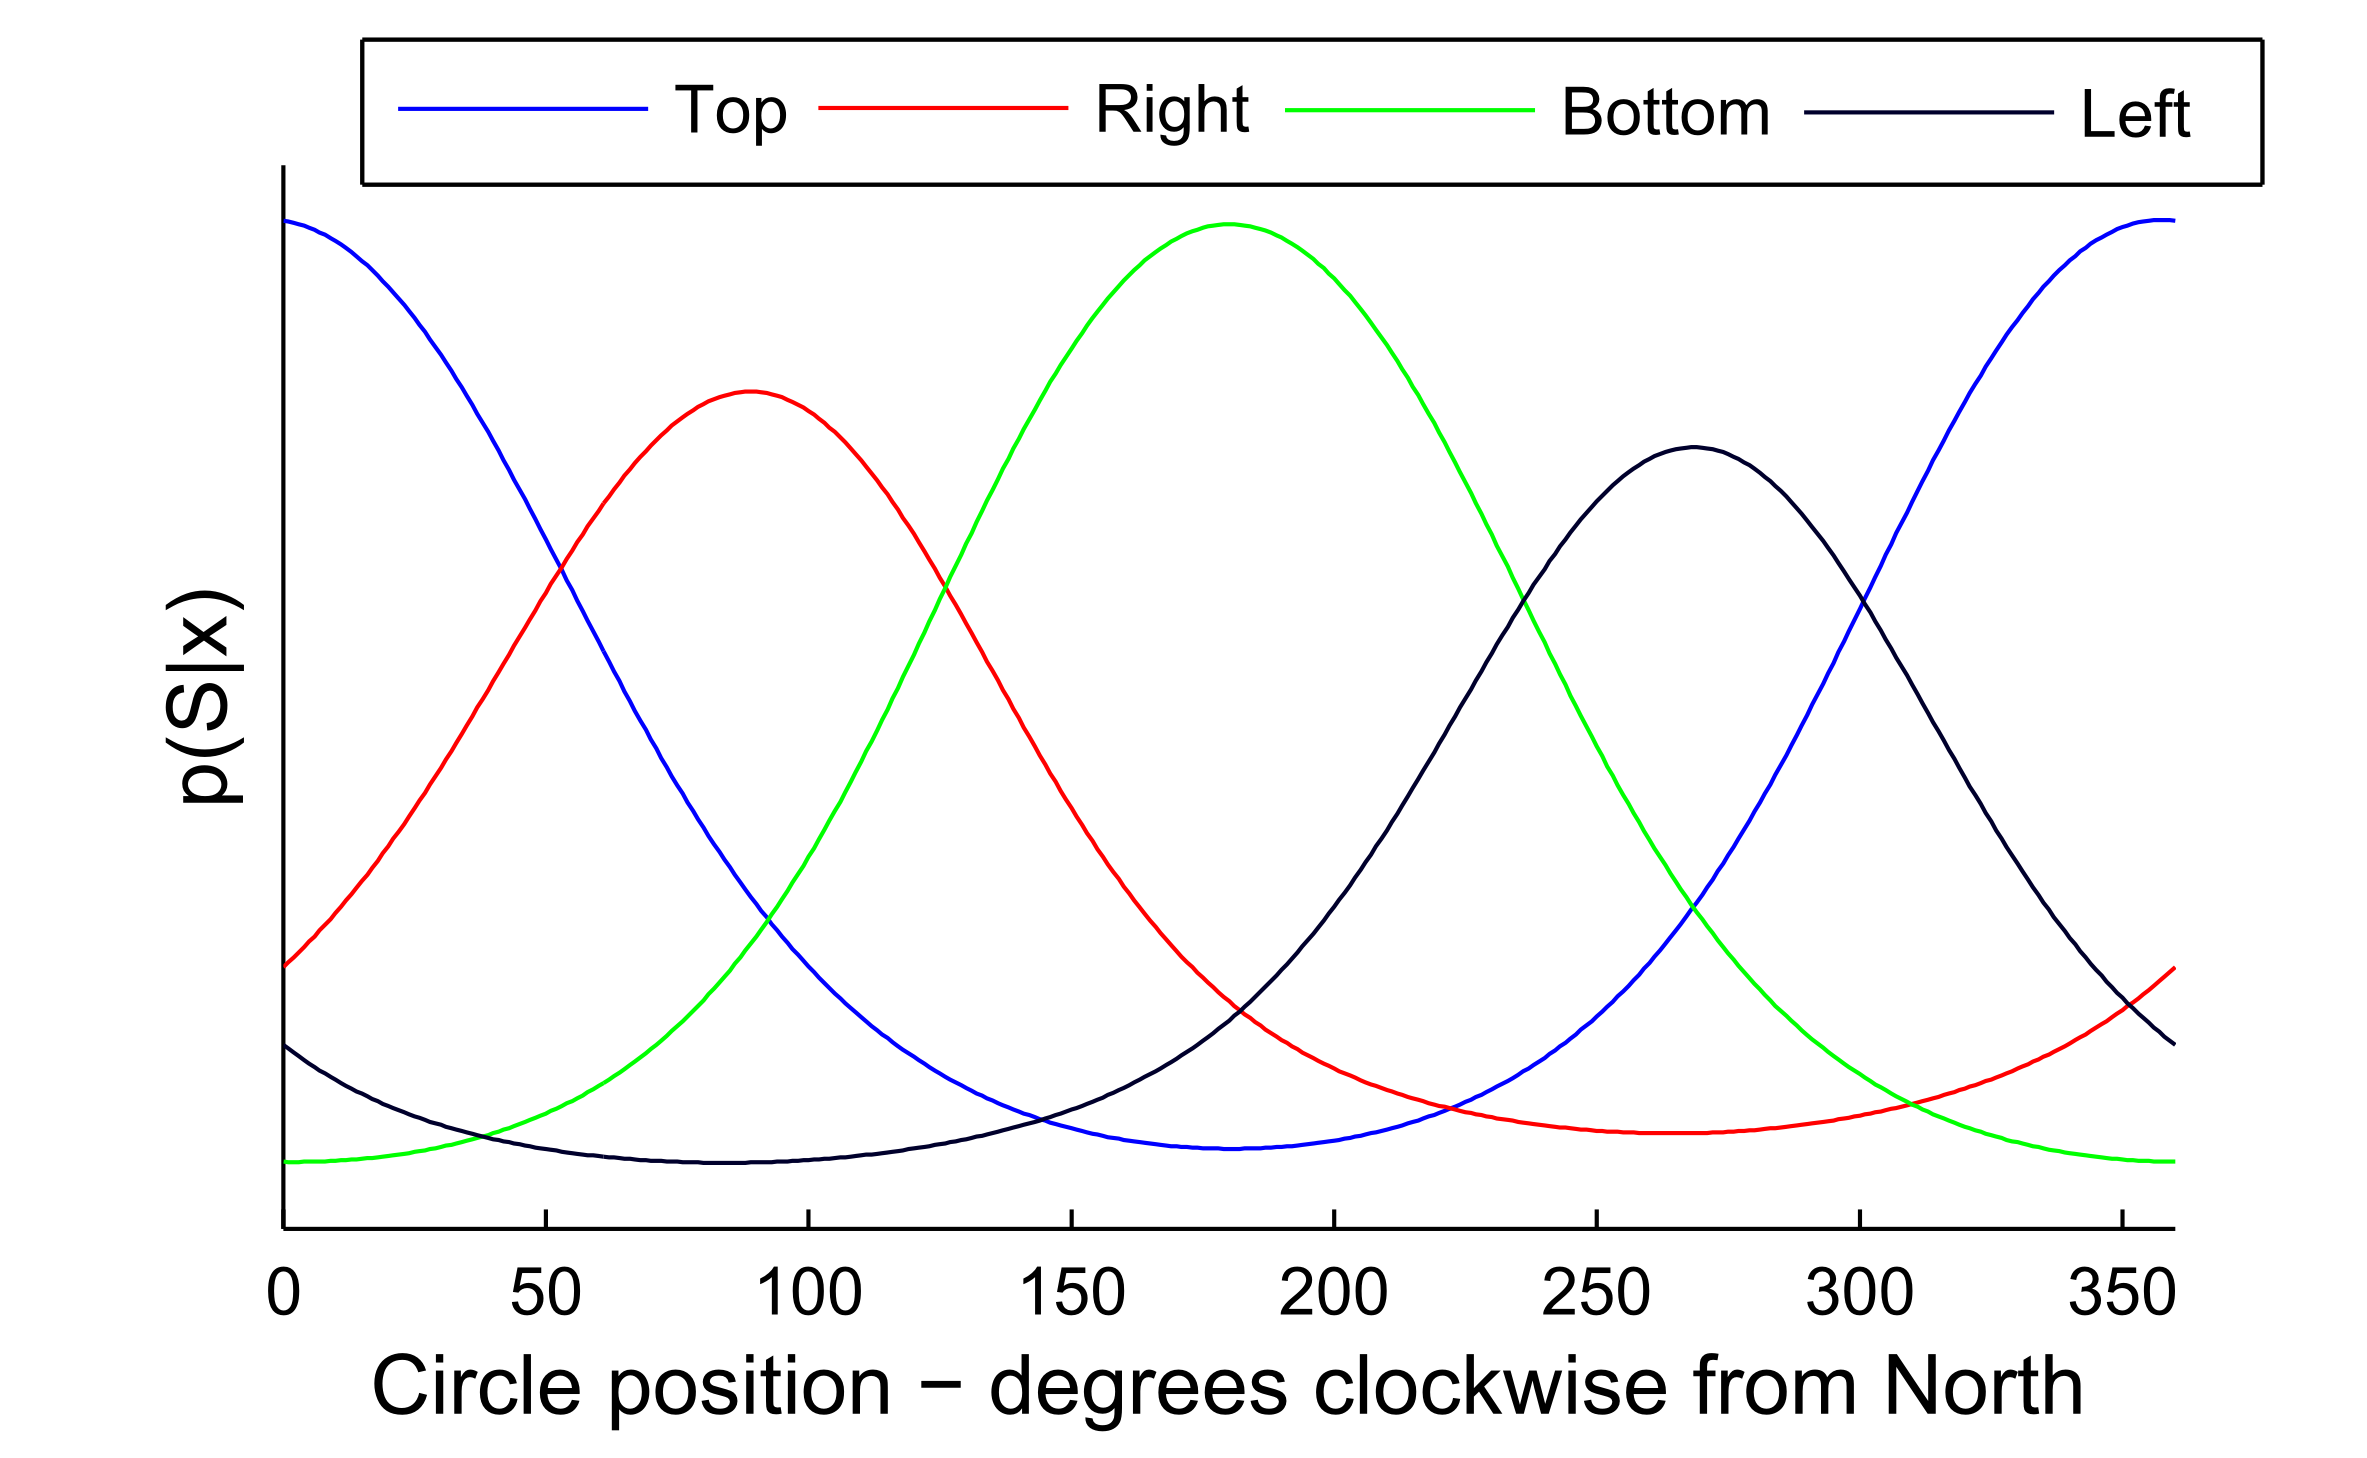
\includegraphics[scale=1]{line_circular_raw_data_softmax.png}
	\caption{The maximum likelihood softmax model for the raw data}
	\label{Figure:cicular_raw_softmax_model_all_responses}
\end{figure}




\begin{figure}
	\centering
	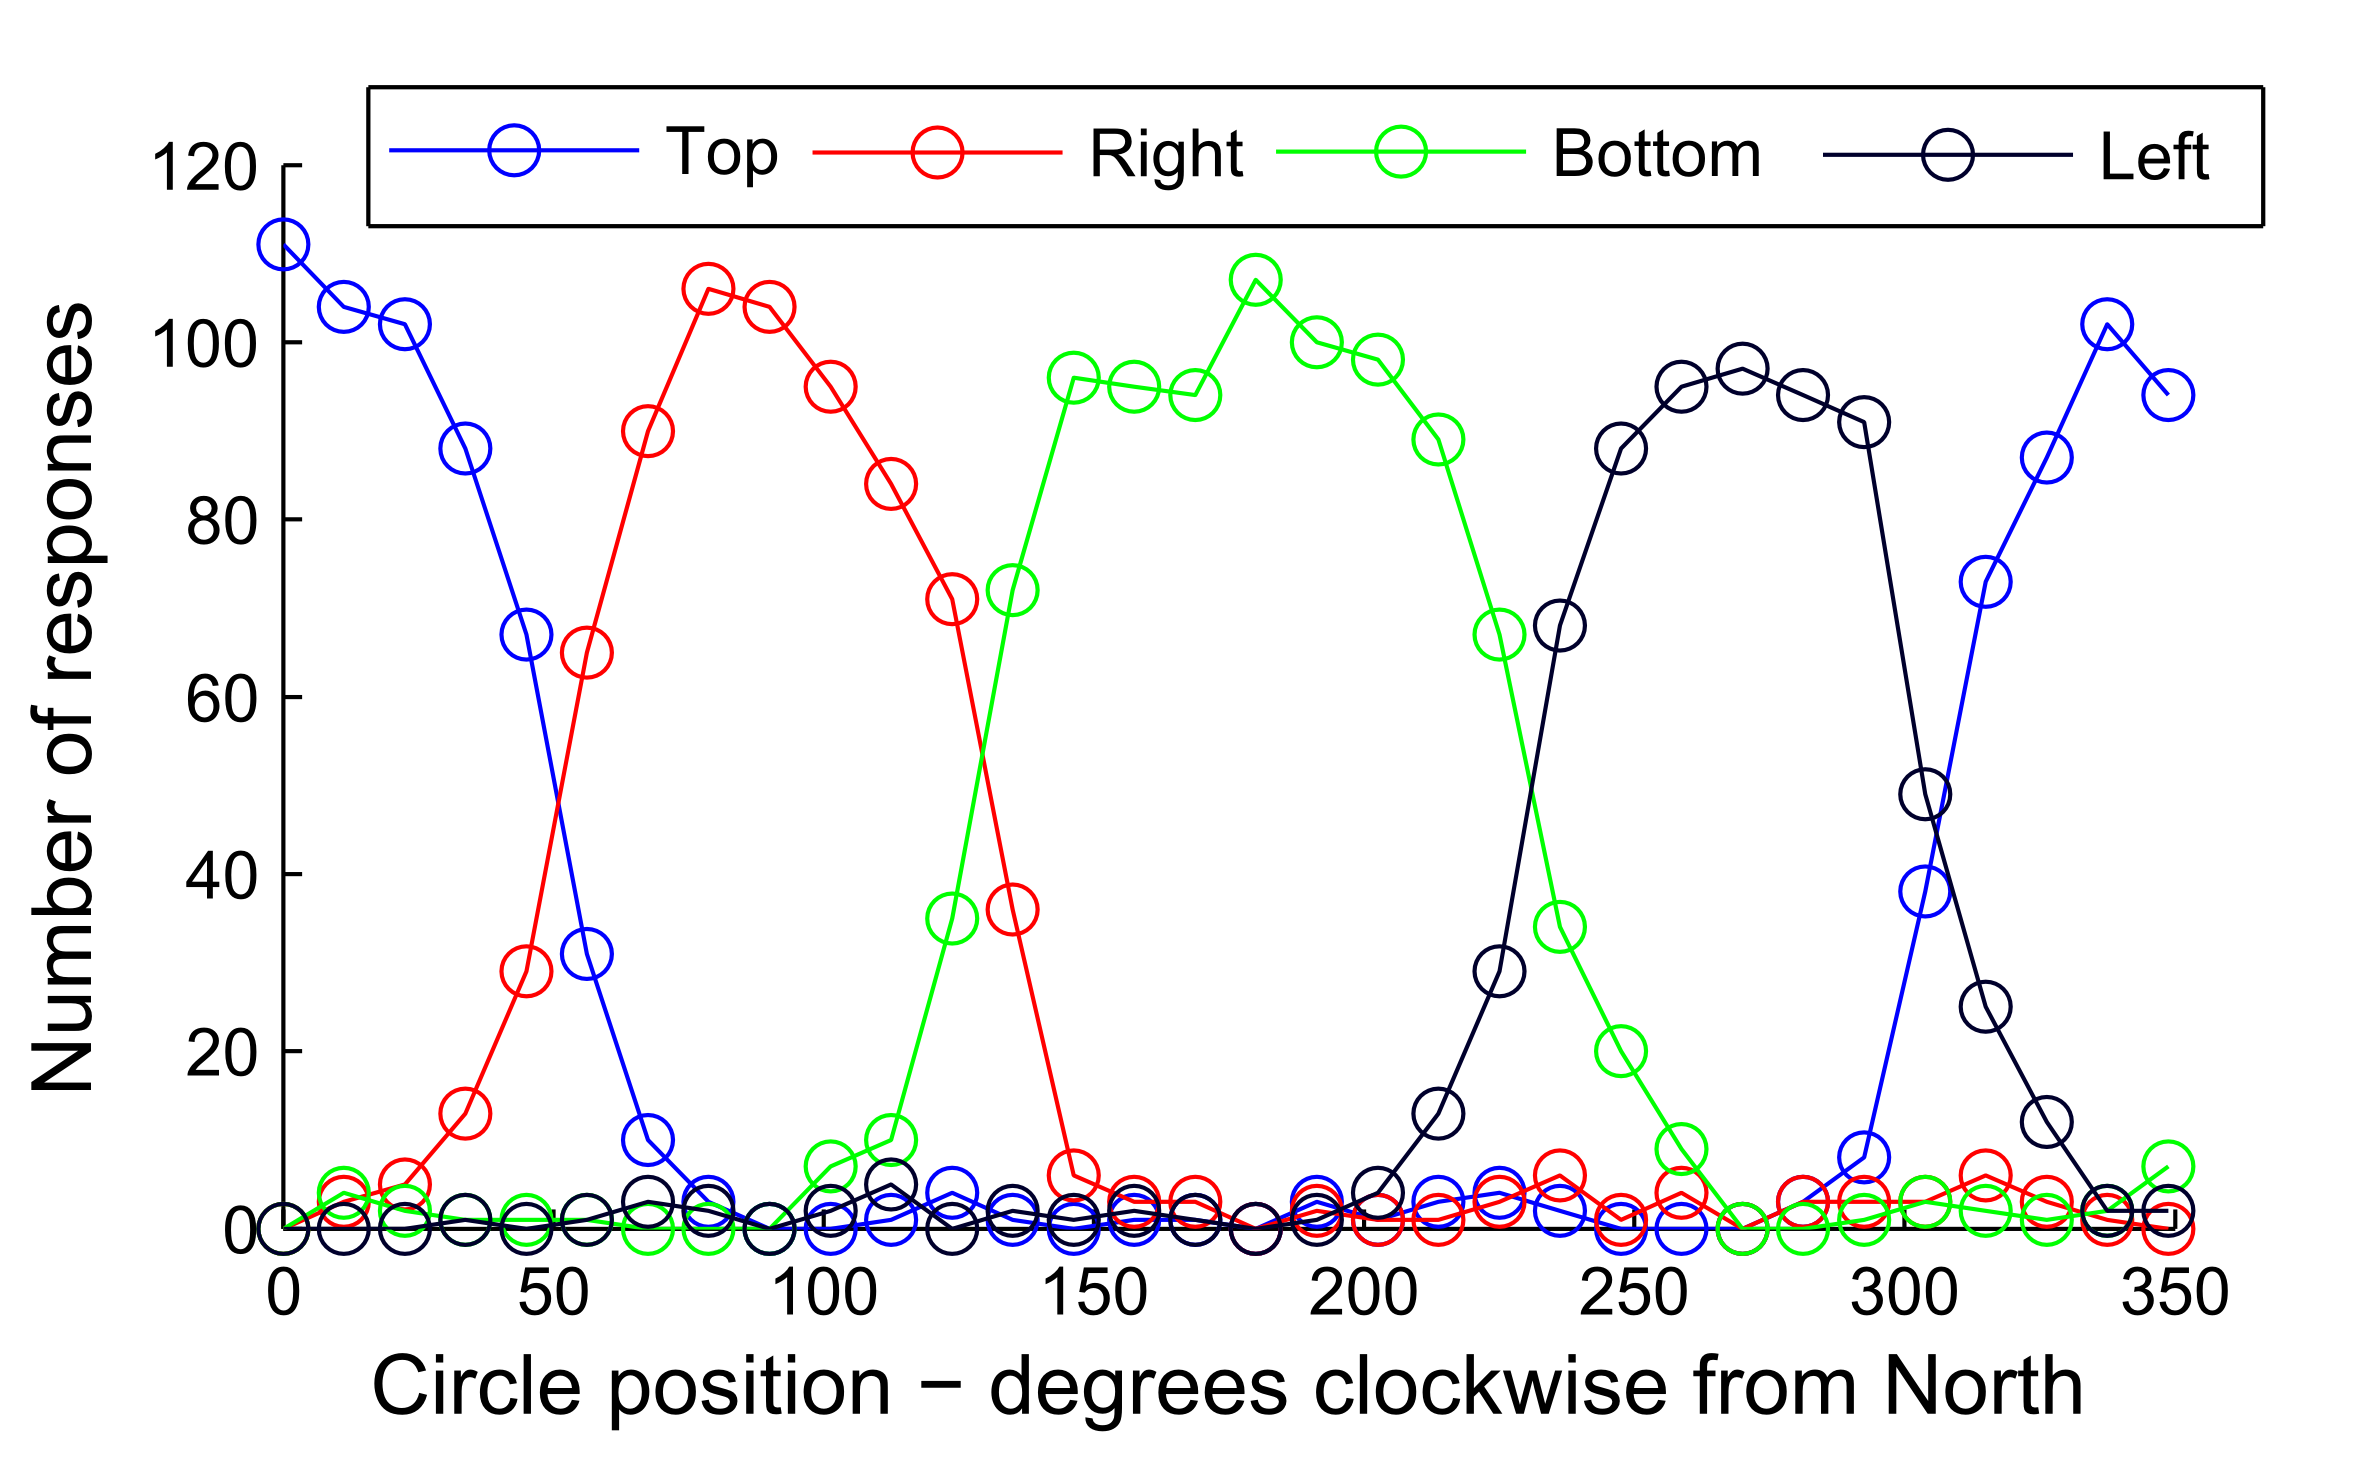
\includegraphics[scale=1]{line_circular_gold_responses.png}
	\caption{The gold data filtered responses. Gold responses were set at 0, 90, 180 and 270. If a worker got a single gold response incorrect, they were filtered out.}
	\label{Figure:cicular_gold_responses}
\end{figure}


\begin{figure}
	\centering
	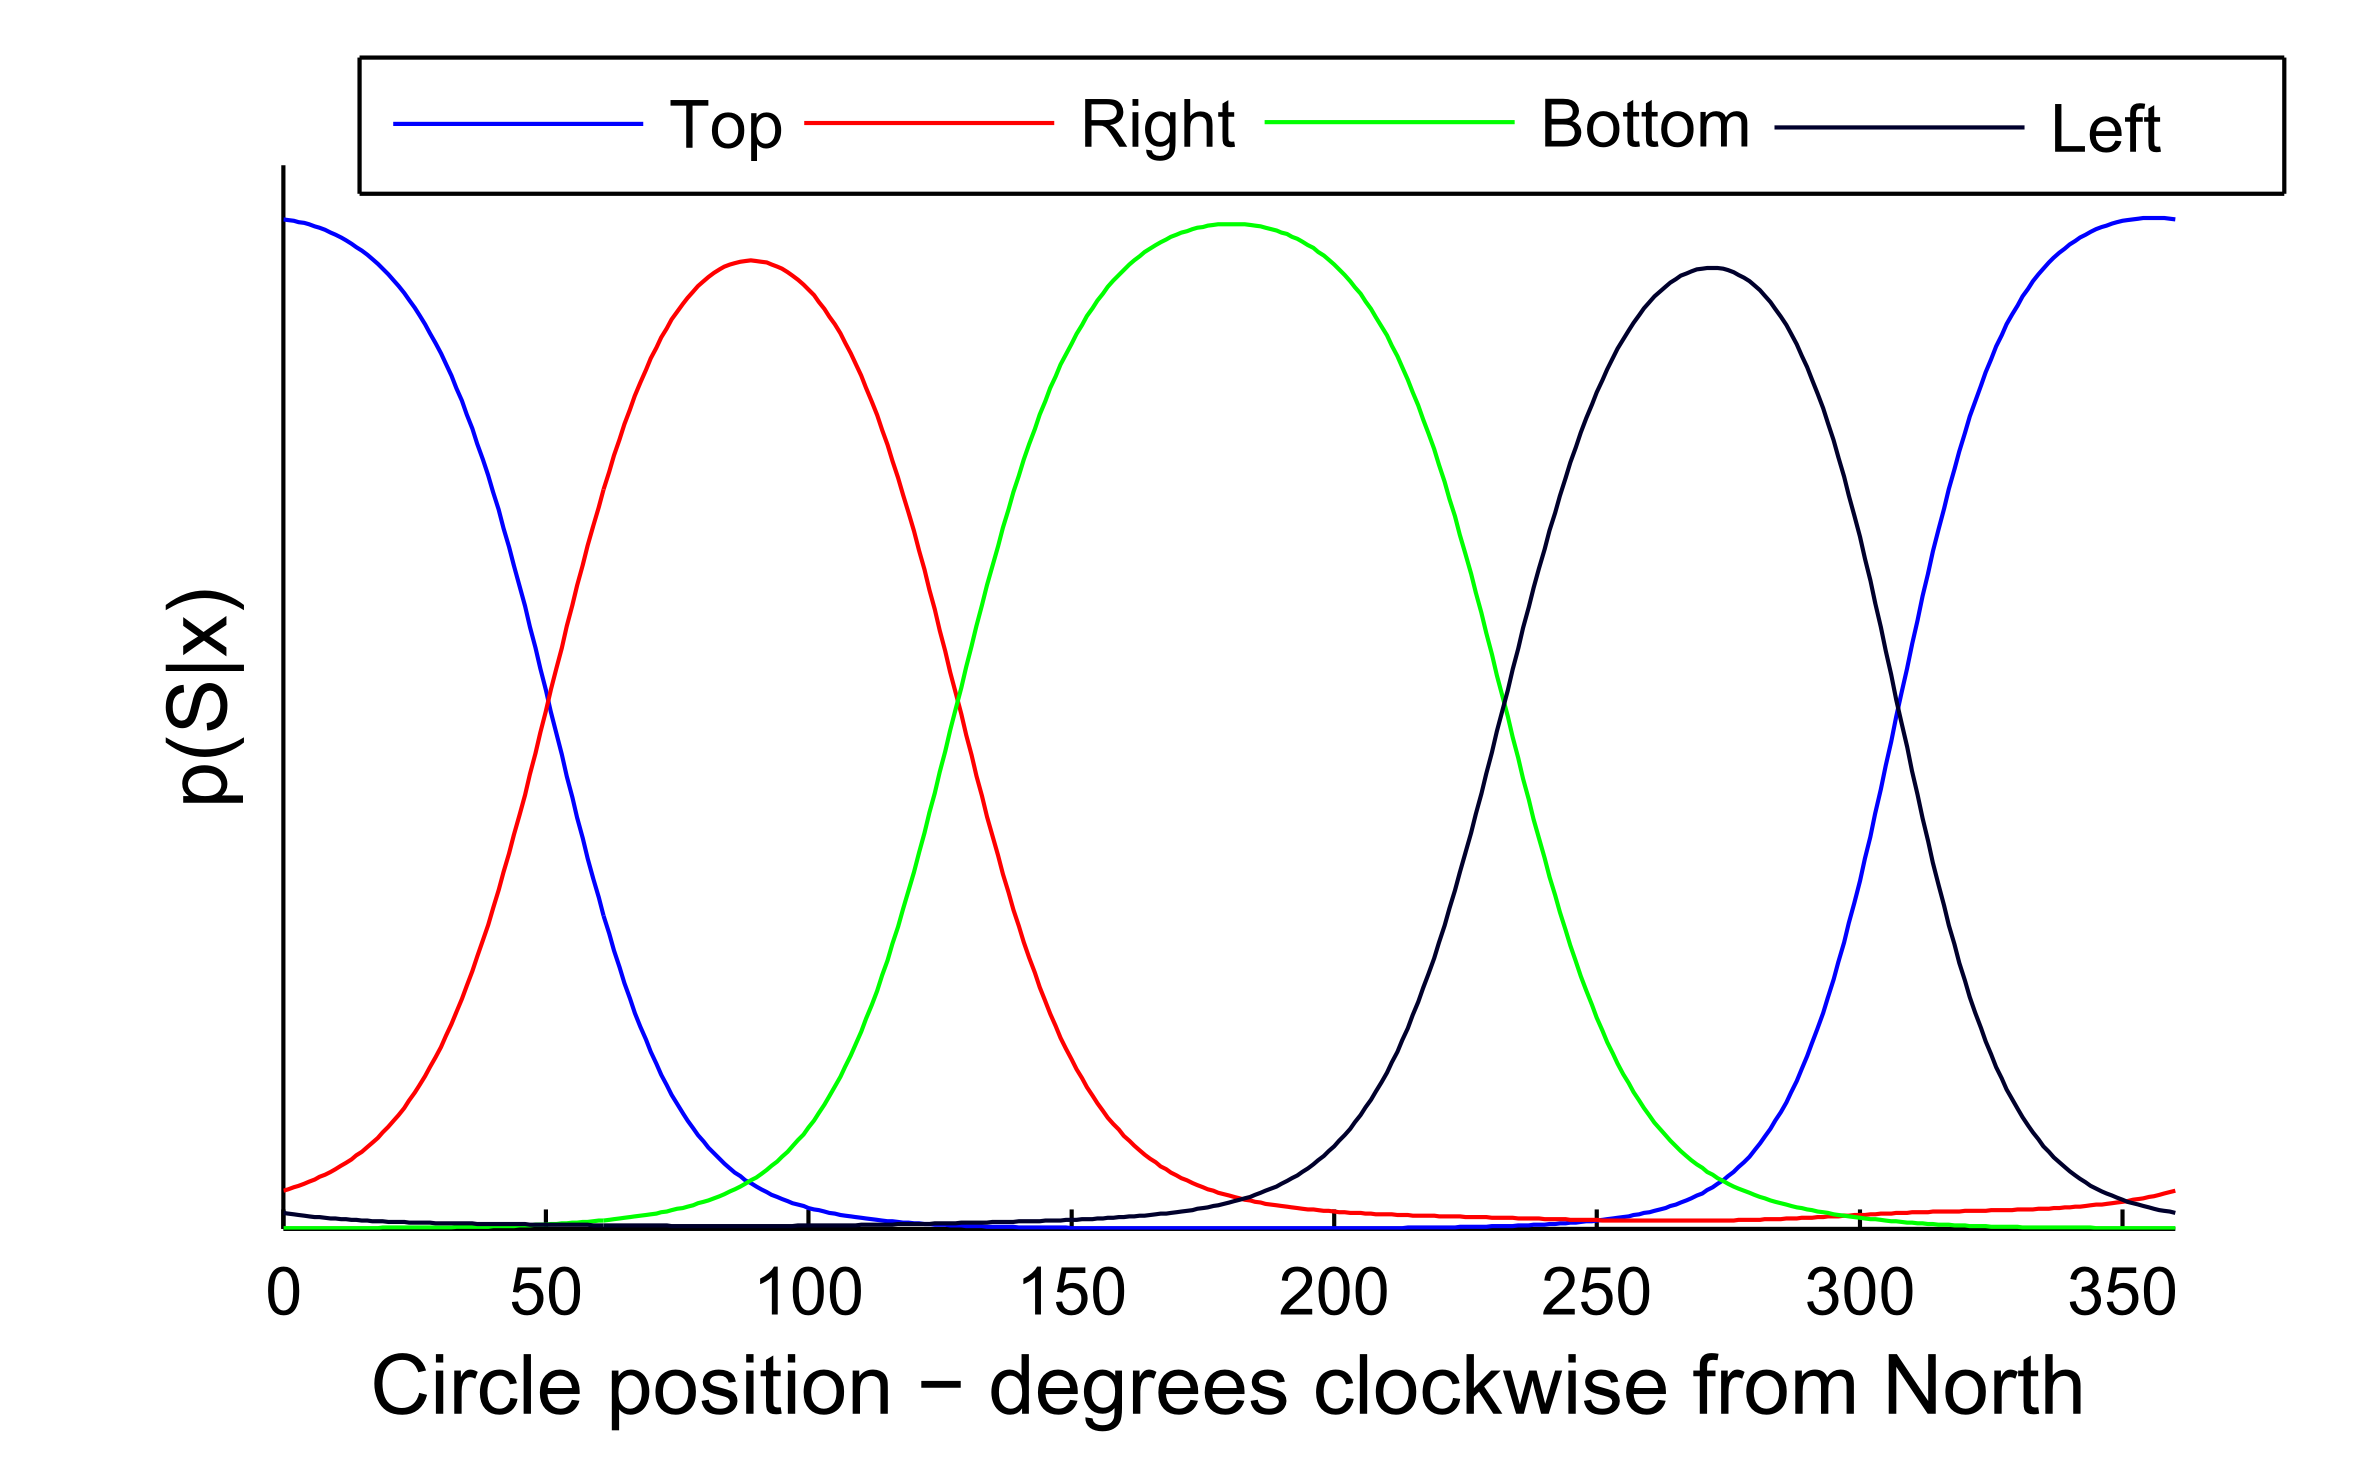
\includegraphics[scale=1]{line_circular_gold_softmax.png}
	\caption{The maximum likelihood softmax model for the gold filtered data.}
	\label{Figure:cicular_gold_softmax_model}
\end{figure}



\section{Data fusion}
\begin{figure}
	\centering
	\begin{subfigure}{7cm}
	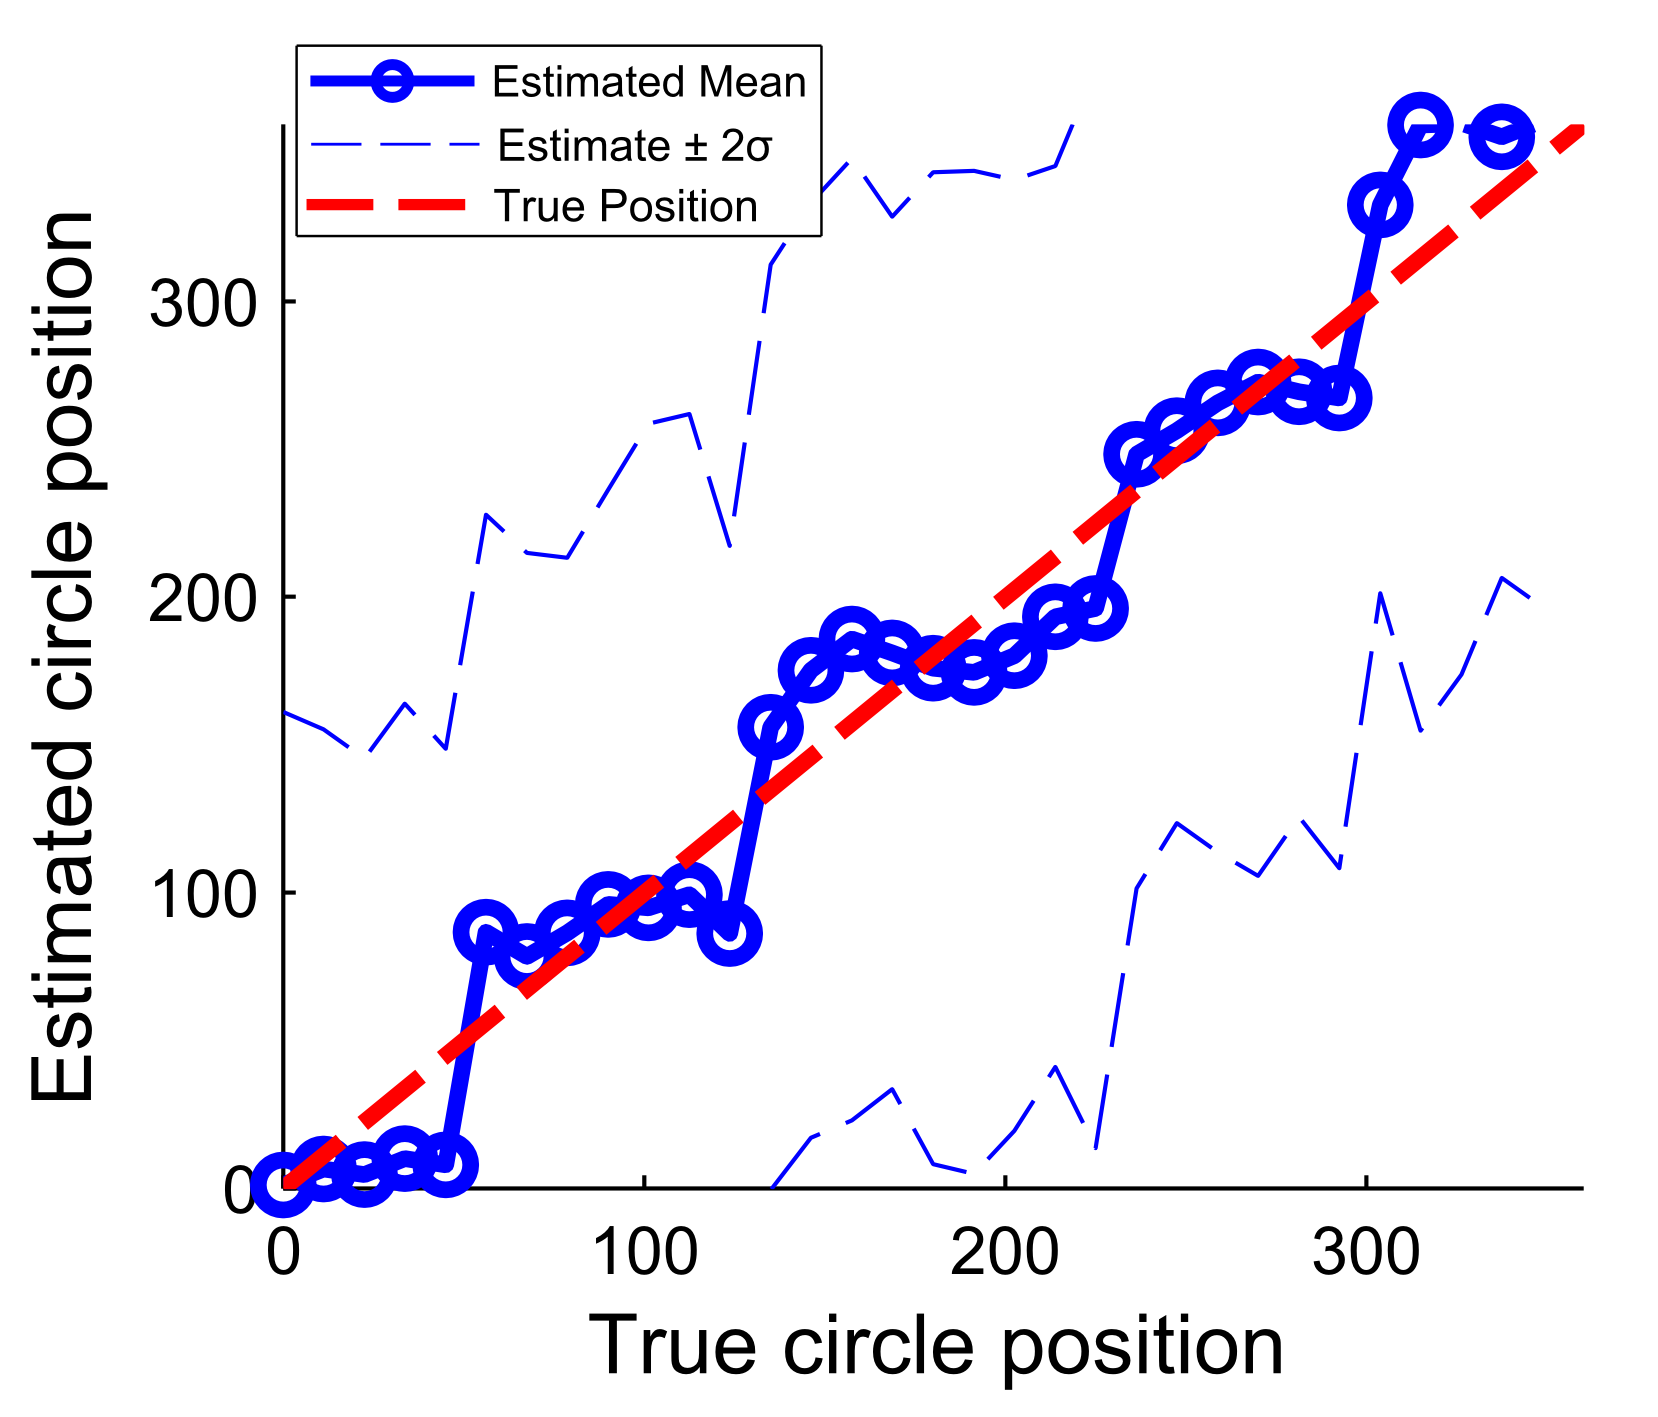
\includegraphics[scale=1]{circular_line_fusion_mean_1report.png}
	\caption{}	
	\label{Figure: circular_fusion_mean_1}
	\end{subfigure}
	\begin{subfigure}{7cm}
	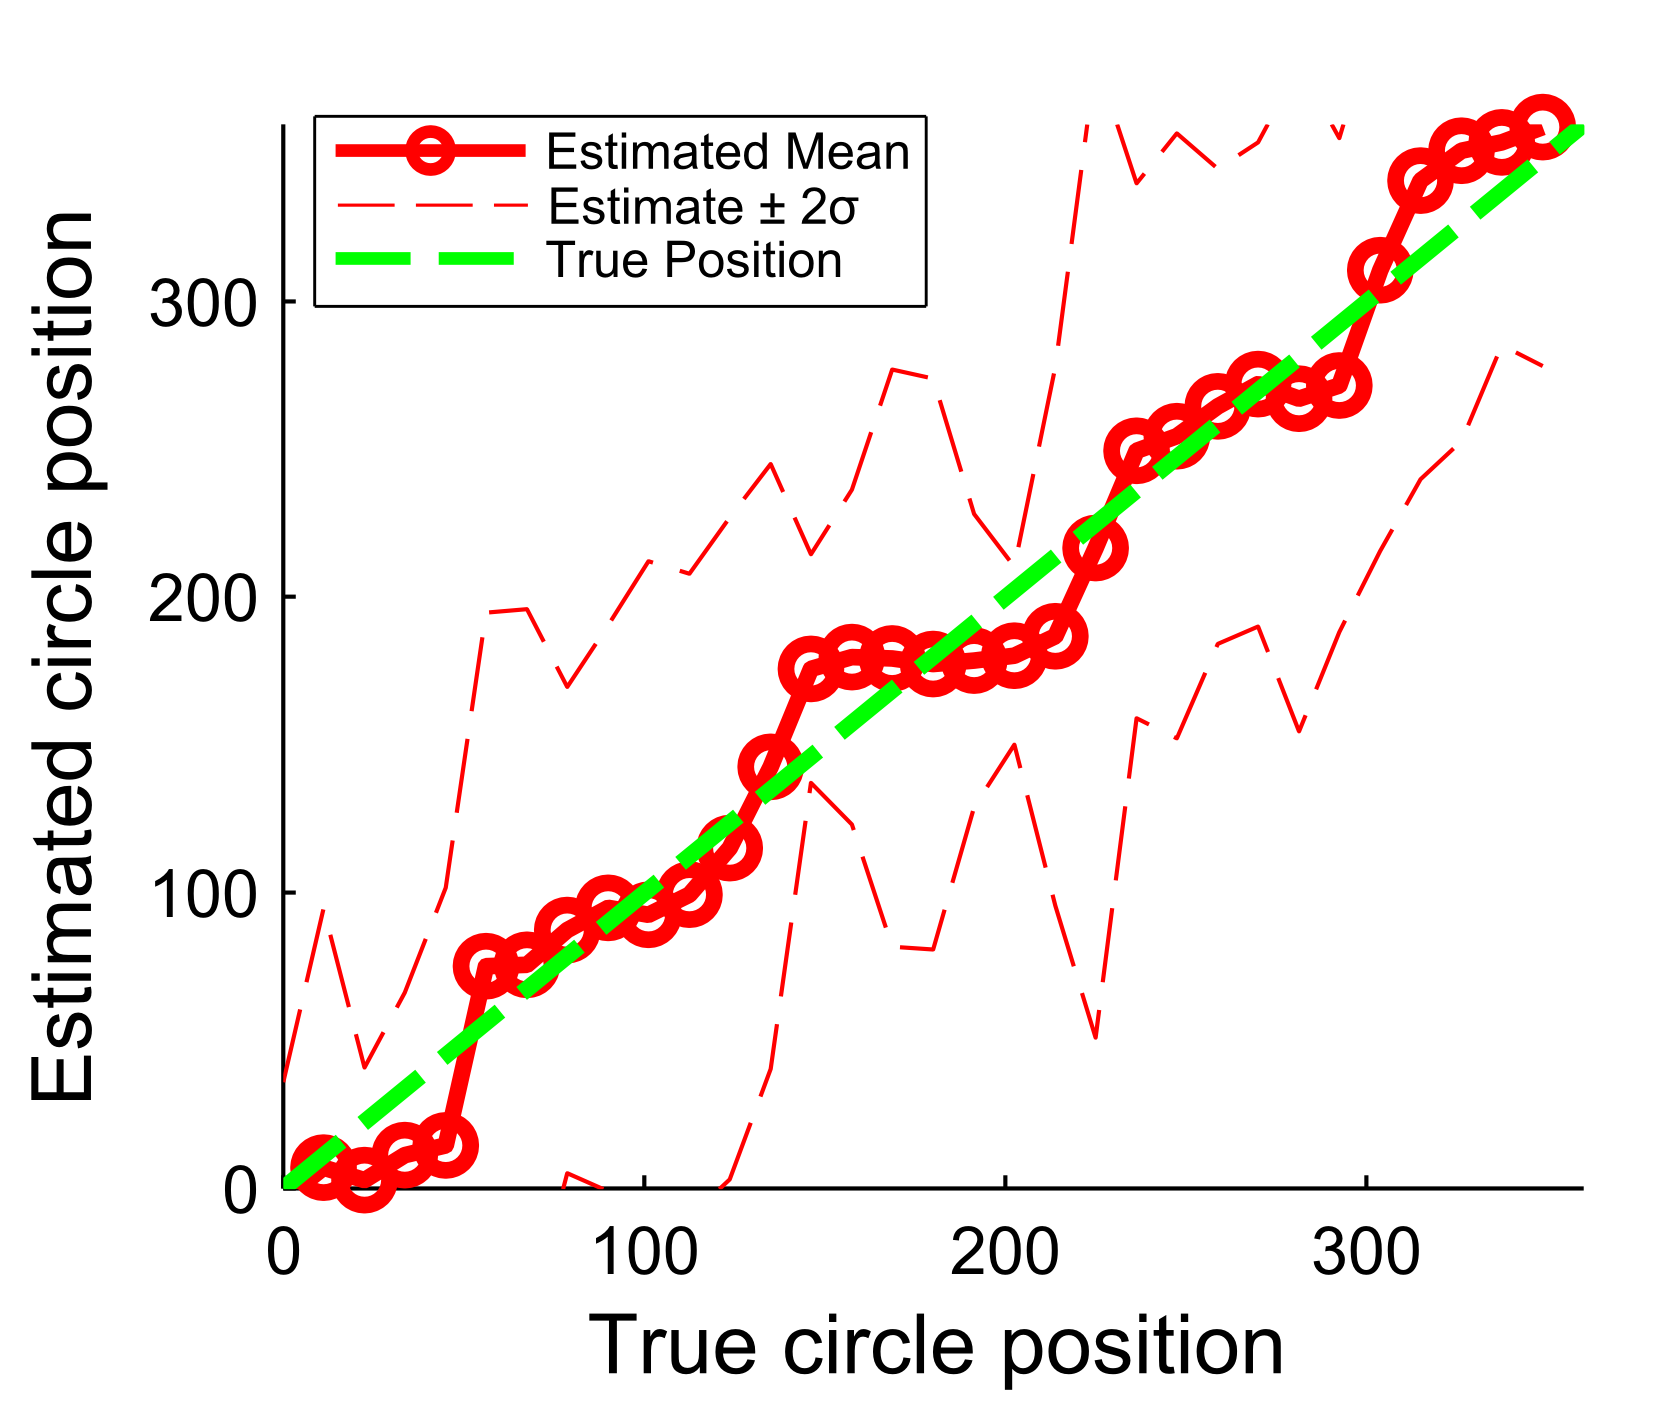
\includegraphics[scale=1]{line_circular_fusion_mean_5.png}
	\caption{}
	\label{Figure: circular_fusion_mean_5}	
	\end{subfigure}\\
	\begin{subfigure}{7cm}
	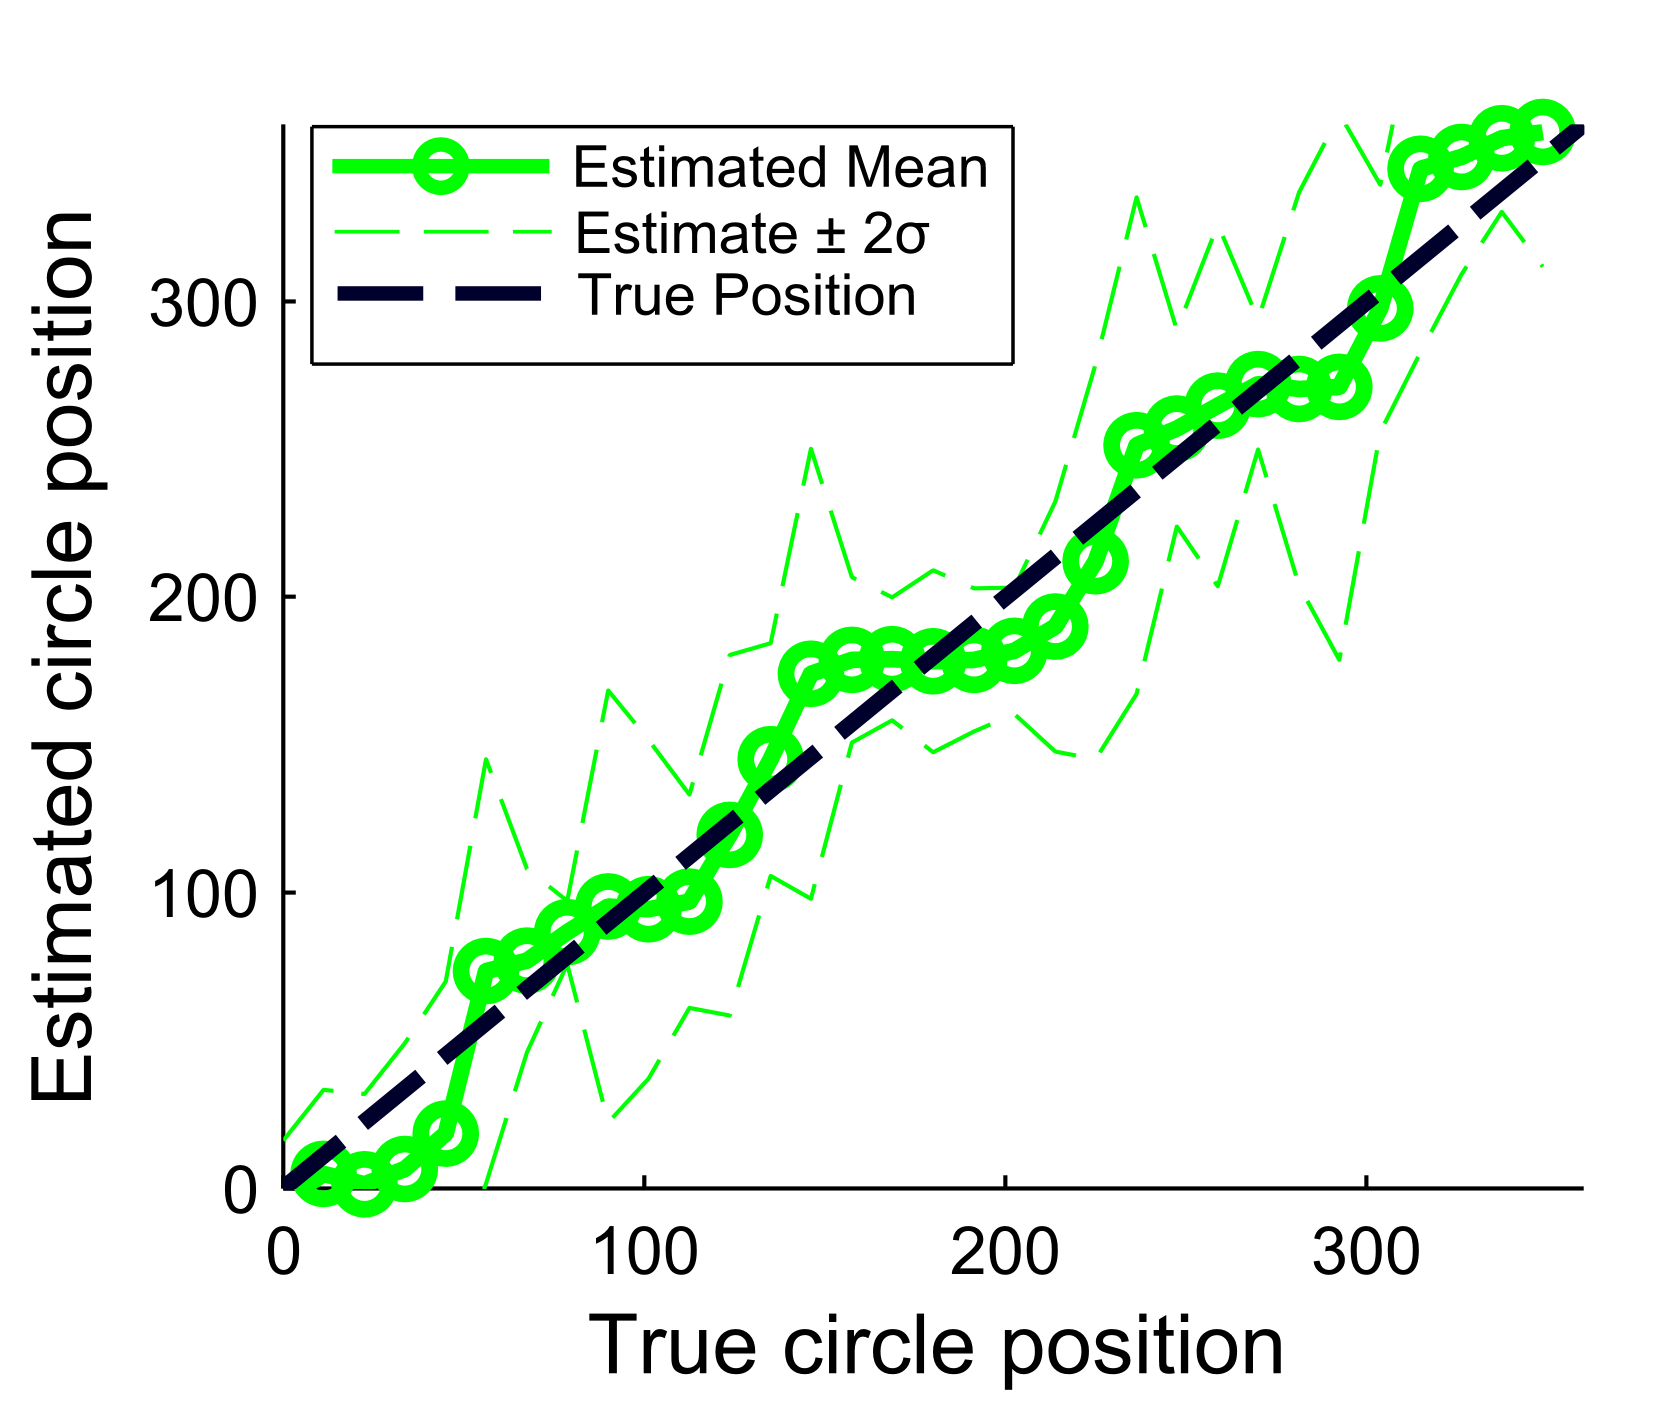
\includegraphics[scale=1]{line_circular_fusion_mean_10.png}
	\caption{}	
	\label{Figure: circular_fusion_mean_10}
	\end{subfigure}
	\begin{subfigure}{7cm}
	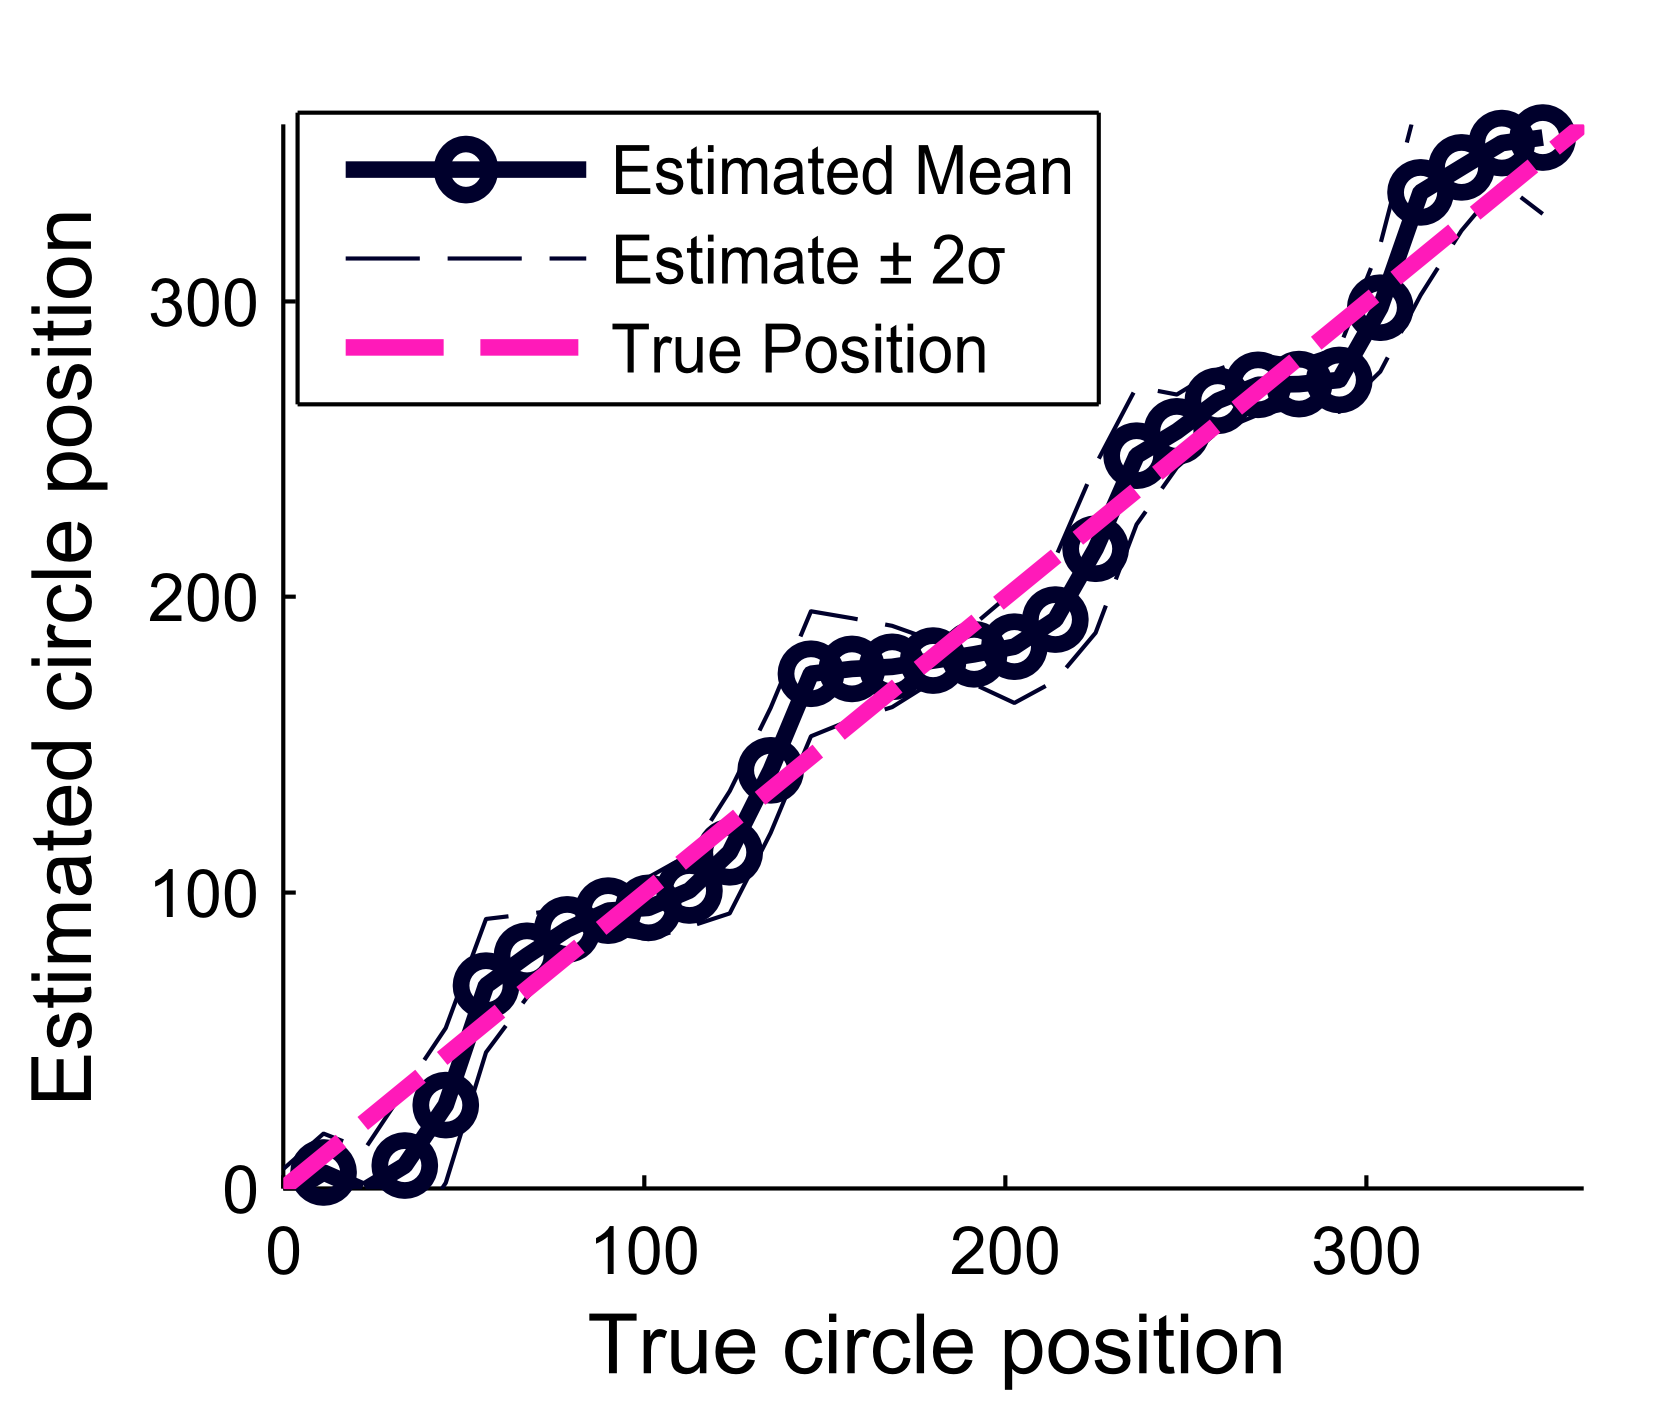
\includegraphics[scale=1]{line_circular_fusion_mean_40.png}
	\caption{}	
	\label{Figure: circular_fusion_mean_40}
	\end{subfigure}
	\label{Figure: circular_fusion_mean}
	\caption{The mean performance of estimating the circle's position from the circular response. The mean line is the expectation value of the posterior distribution taken from 50 simulations. The standard deviation is for the spread of expectation values over the simulations - not the spread in individual posteriors. The data was collected for varying numbers of responses with \subref{Figure: circular_fusion_mean_1}) 1 response \subref{Figure: circular_fusion_mean_5}) 5 responses \subref{Figure: circular_fusion_mean_10}) 10 responses \subref{Figure: circular_fusion_mean_40})40 responses}
\end{figure}


\begin{figure}
	\centering
	\begin{subfigure}{7cm}
	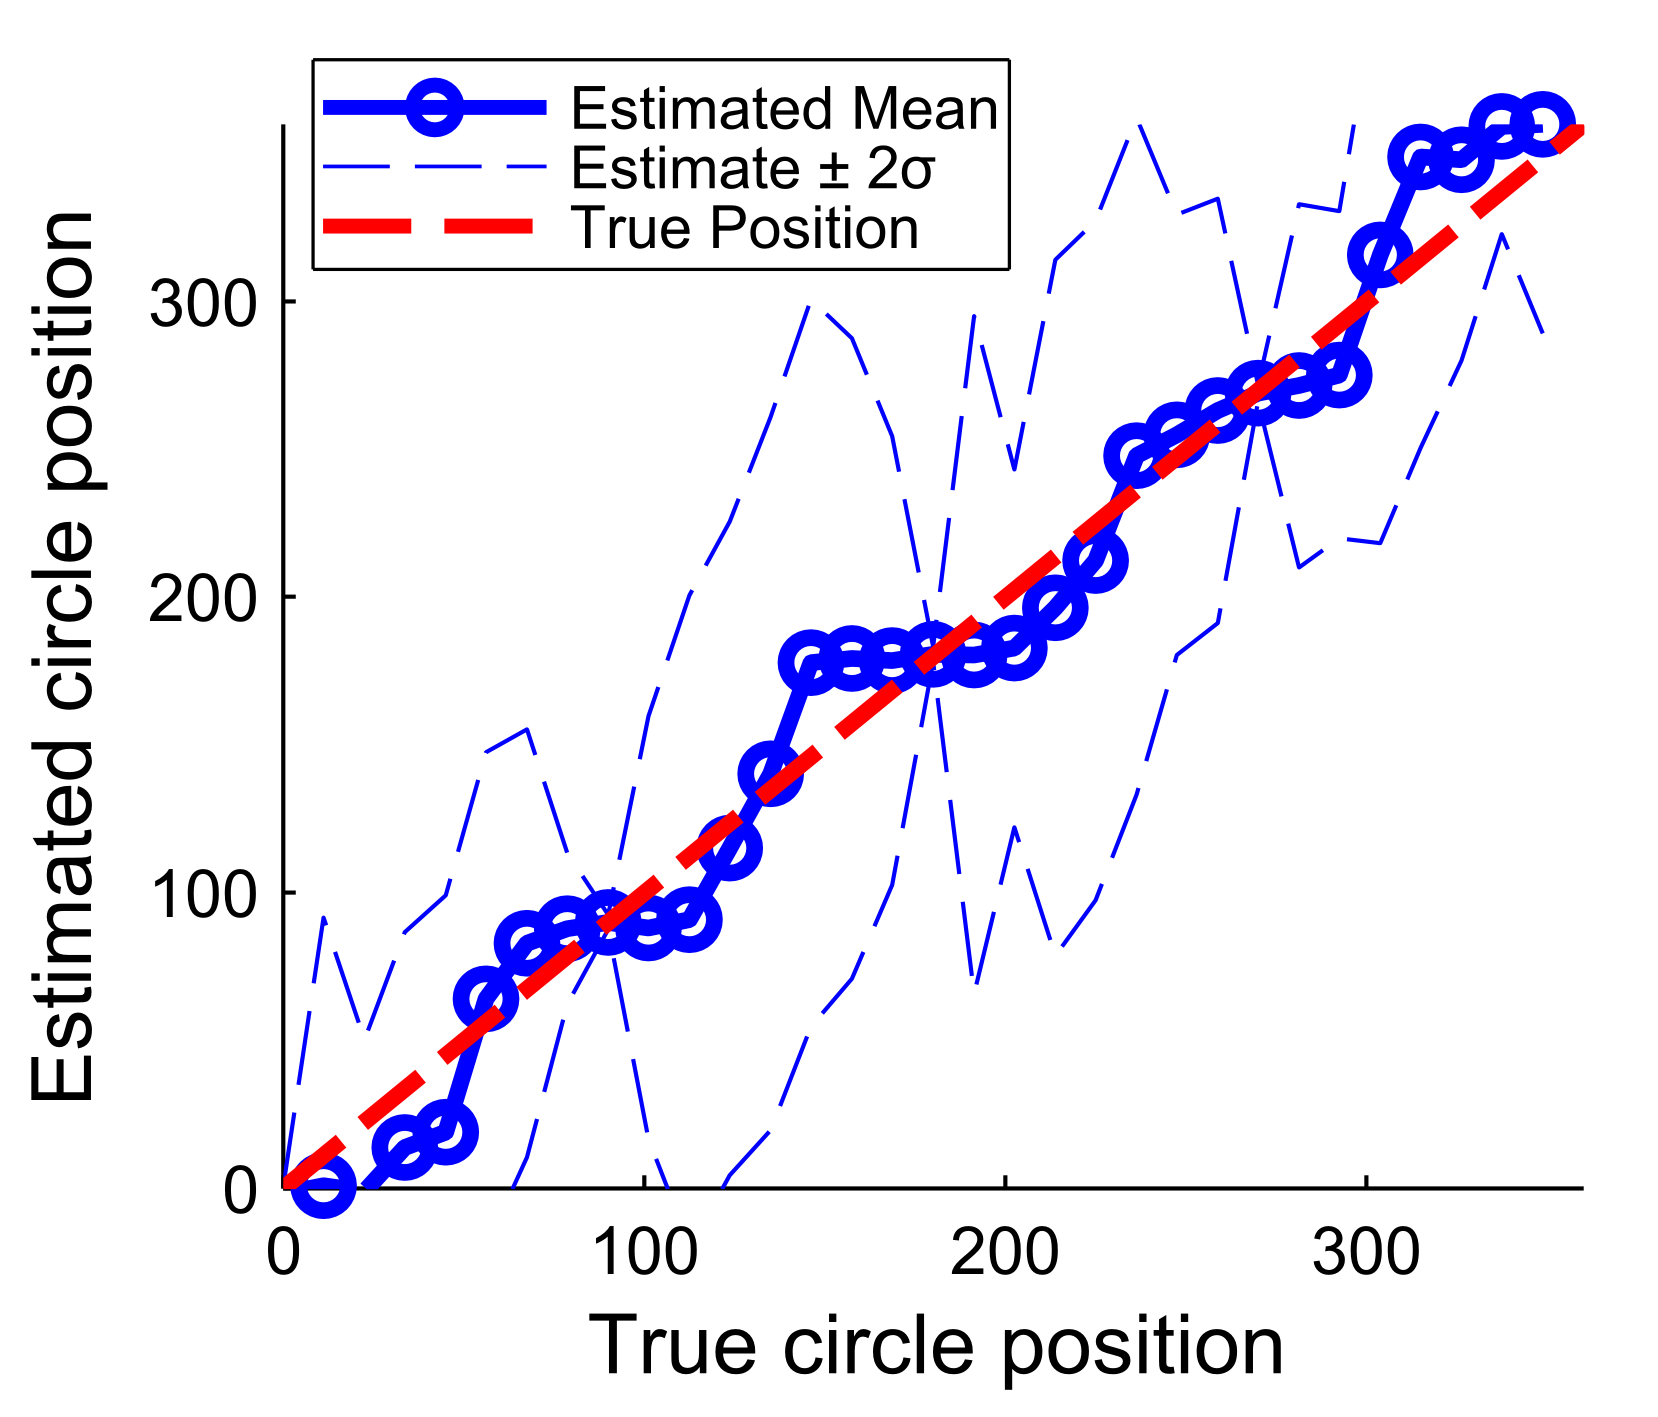
\includegraphics[scale=1]{circular_line_fusion_mean_1report_gold.png}
	\caption{}	
	\label{Figure: circular_fusion_mean_1_gold}
	\end{subfigure}
	\begin{subfigure}{7cm}
	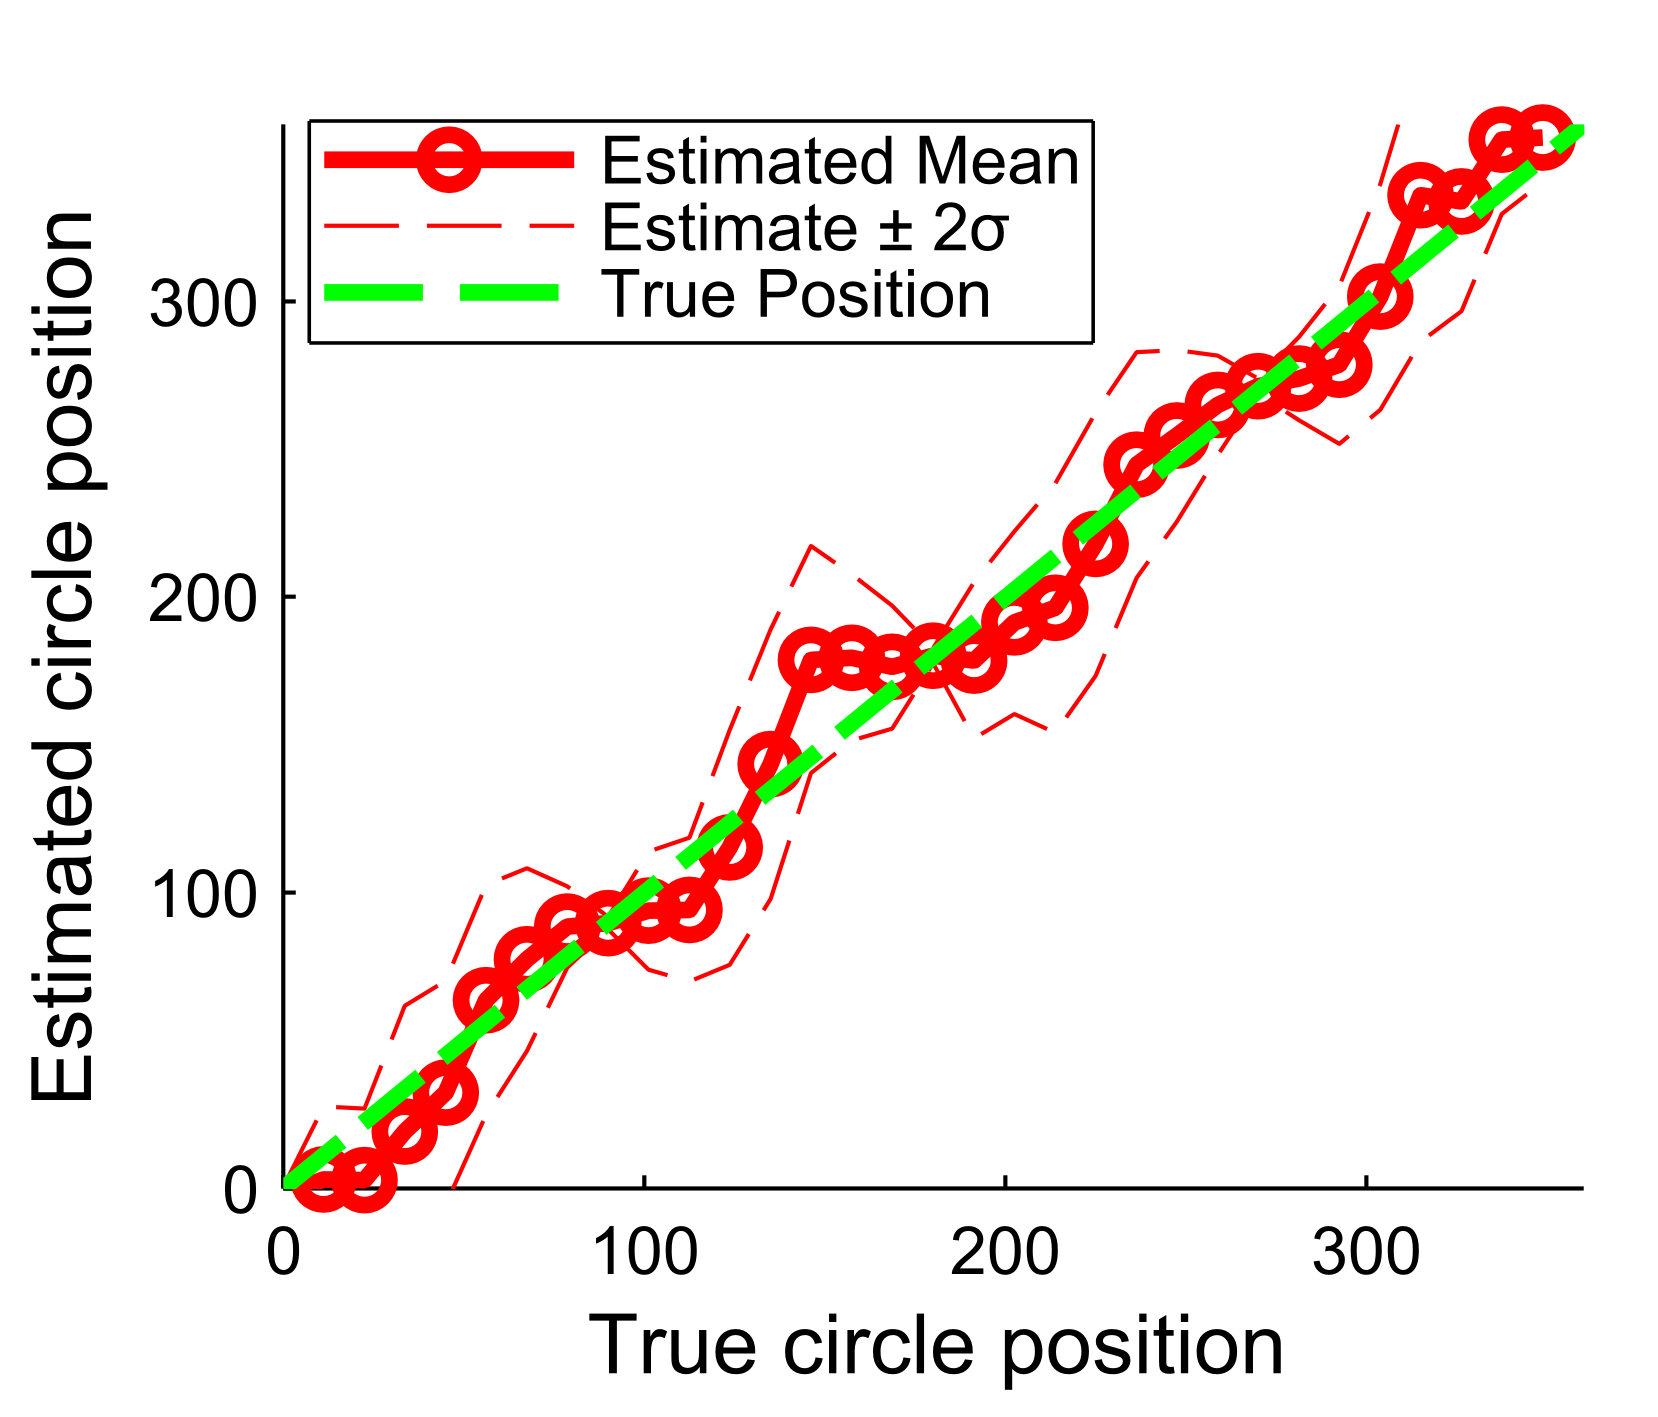
\includegraphics[scale=1]{line_circular_fusion_mean_5_gold.png}
	\caption{}
	\label{Figure: circular_fusion_mean_5_gold}	
	\end{subfigure}\\
	\begin{subfigure}{7cm}
	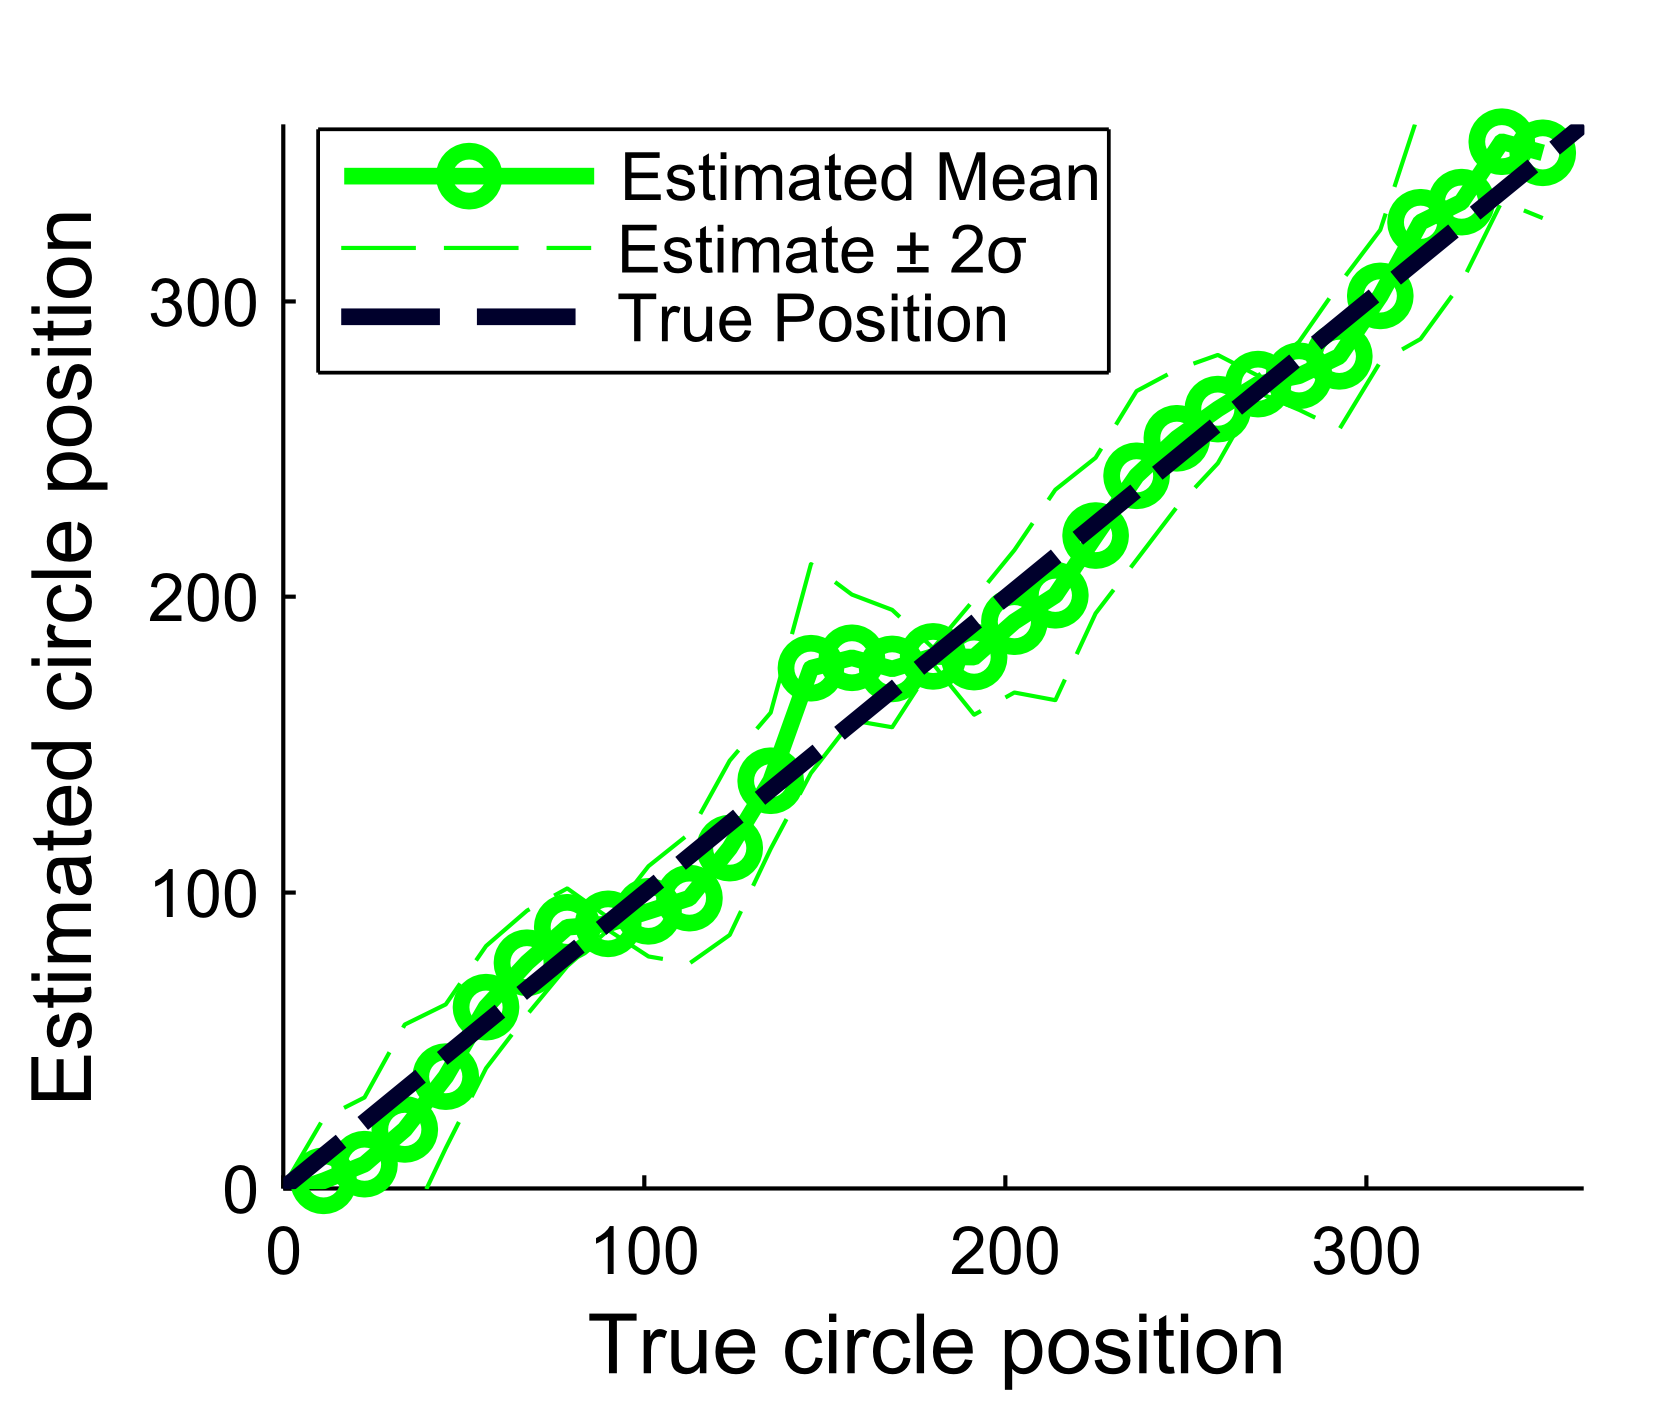
\includegraphics[scale=1]{line_circular_fusion_mean_10_gold.png}
	\caption{}	
	\label{Figure: circular_fusion_mean_10_gold}
	\end{subfigure}
	\begin{subfigure}{7cm}
	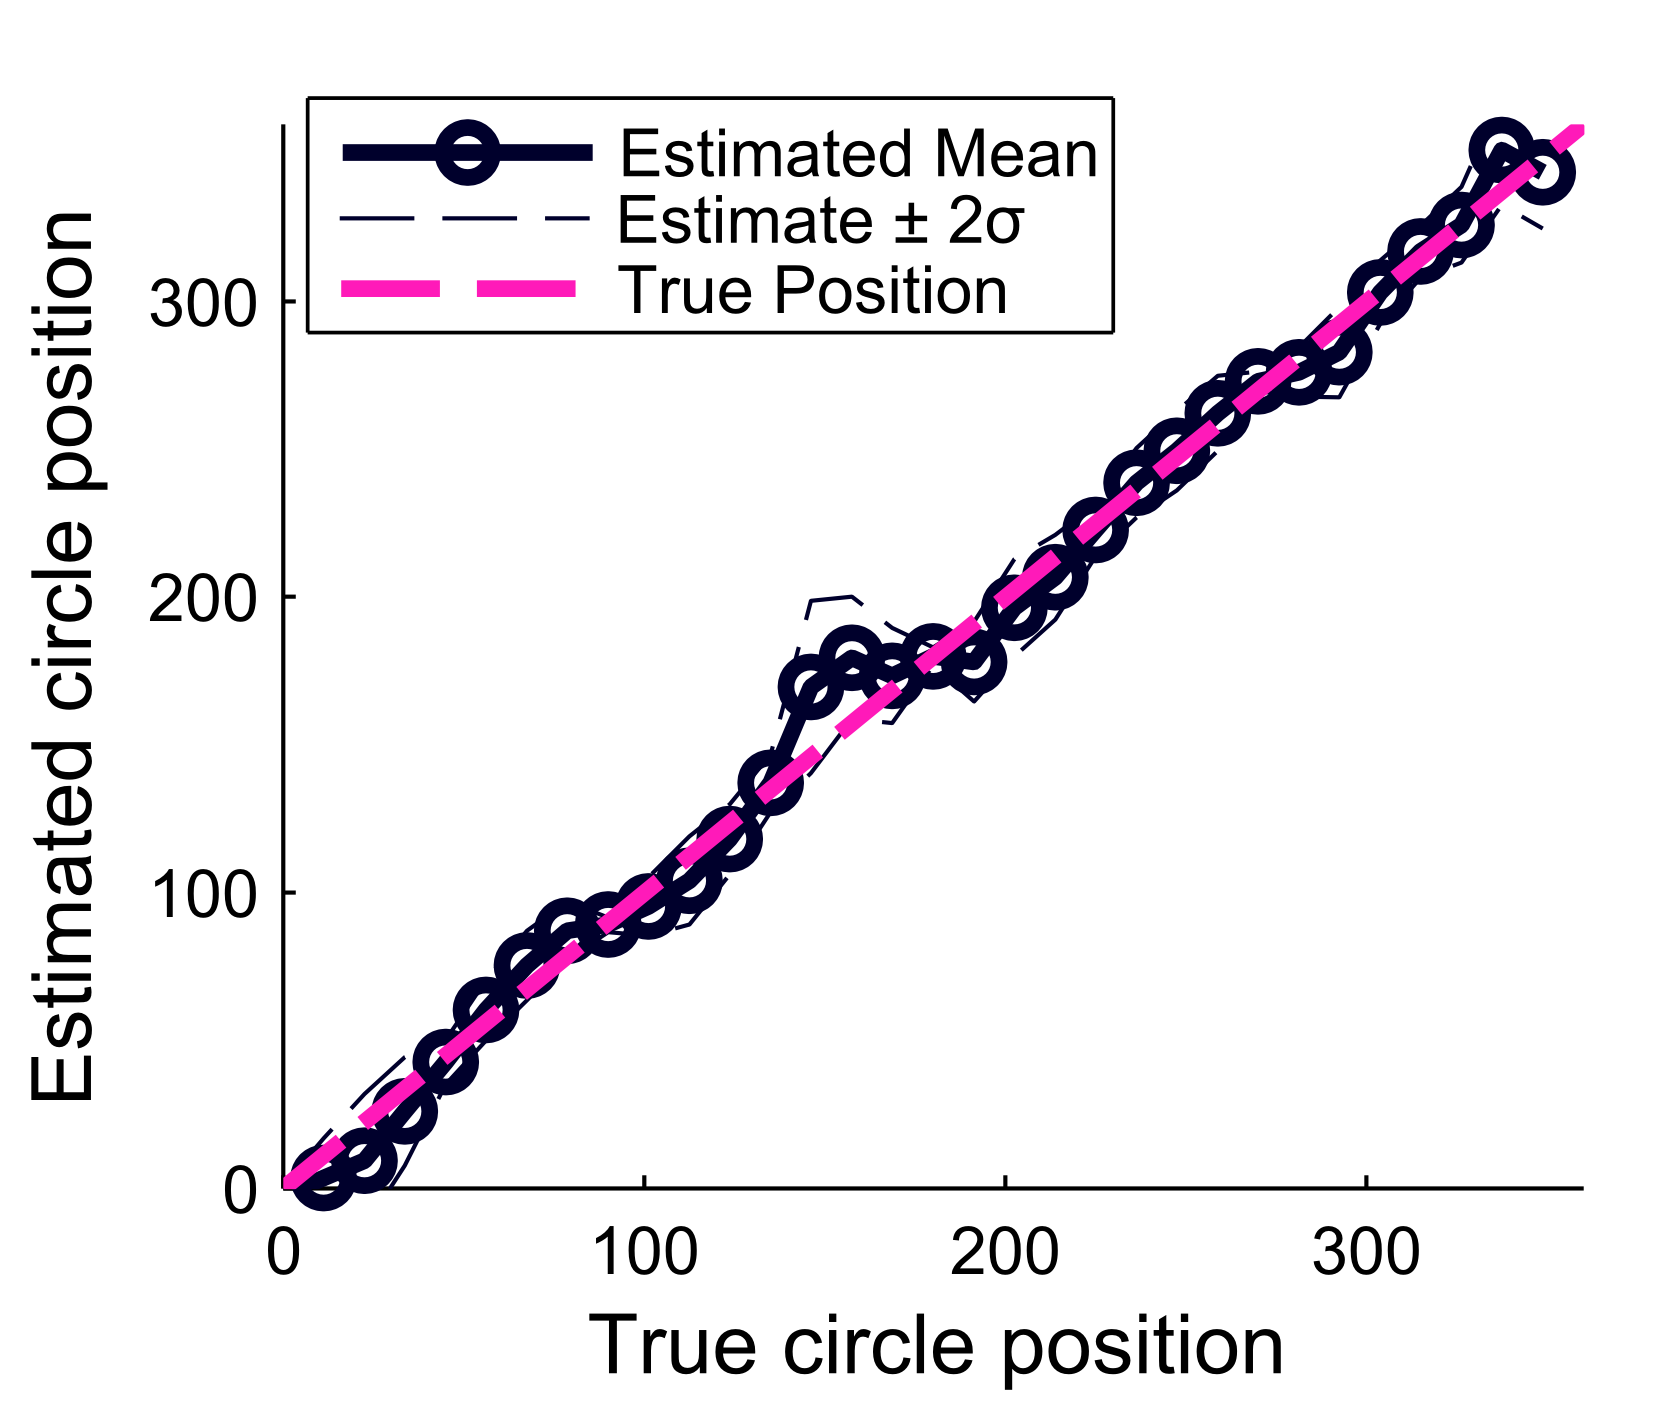
\includegraphics[scale=1]{line_circular_fusion_mean_40_gold.png}
	\caption{}	
	\label{Figure: circular_fusion_mean_40_gold}
	\end{subfigure}
	\label{Figure: circular_fusion_mean_gold}
	\caption{The mean performance of estimating the circle's position from the circular response gold data. The mean line is the expectation value of the posterior distribution taken from 50 simulations. The standard deviation is for the spread of expectation values over the simulations - not the spread in individual posteriors. The data was collected for varying numbers of responses with \subref{Figure: circular_fusion_mean_1_gold}) 1 response \subref{Figure: circular_fusion_mean_5_gold}) 5 responses \subref{Figure: circular_fusion_mean_10_gold}) 10 responses \subref{Figure: circular_fusion_mean_40_gold})40 responses}
\end{figure}